\subsection{Упражнение 1}

Оцените высоты тона вокального чирпа для нескольких времён начала сегмента.

\begin{lstlisting}[language=Python]
if not os.path.exists('28042__bcjordan__voicedownbew.wav'):
    !wget https://github.com/AllenDowney/ThinkDSP/raw/master/code/28042__bcjordan__voicedownbew.wav
from thinkdsp import read_wave
wave = read_wave('28042__bcjordan__voicedownbew.wav')
wave.normalize()
wave.make_audio()

duration = 0.01
segment1 = wave.segment(start=0.5, duration=duration)
segment1.plot()
segment2 = wave.segment(start=0.6, duration=duration)
segment2.plot()
segment3 = wave.segment(start=0.7, duration=duration)
segment3.plot()
\end{lstlisting}
\begin{figure}[H]
	\begin{center}
		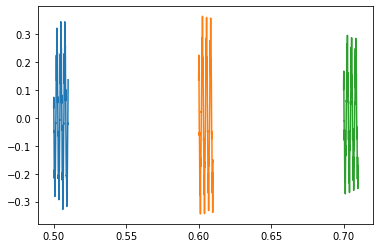
\includegraphics[scale=1]{fig/lab05/lab05_1.png}
		\caption{График сегментов}
	\end{center}
\end{figure}

Используем автокореляцию.

\begin{lstlisting}[language=Python]
lags1, corrs1 = autocorr(segment1)
plt.plot(lags1, corrs1, color='black')
decorate(xlabel='Lag', ylabel='Correlation', ylim=[-1, 1])

lags2, corrs2 = autocorr(segment2)
plt.plot(lags2, corrs2)
decorate(xlabel='Lag', ylabel='Correlation', ylim=[-1, 1])

lags3, corrs3 = autocorr(segment3)
plt.plot(lags3, corrs3, color='red')
decorate(xlabel='Lag', ylabel='Correlation', ylim=[-1, 1])
\end{lstlisting}
\begin{figure}[H]
	\begin{center}
		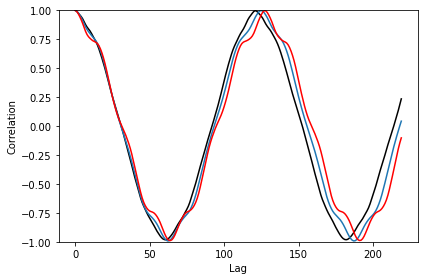
\includegraphics[scale=1]{fig/lab05/lab05_2.png}
		\caption{Автокорреляция сигналов}
	\end{center}
\end{figure}

Вычислим lag

\begin{lstlisting}[language=Python]
low = 50
high = 200
lag1 = np.array(corrs1[low:high]).argmax() + low
lag2 = np.array(corrs2[low:high]).argmax() + low
lag3 = np.array(corrs3[low:high]).argmax() + low

lag1,lag2, lag3
\end{lstlisting}
\begin{lstlisting}
(121, 125, 127)
\end{lstlisting}

Вычислим периоды

\begin{lstlisting}[language=Python]
period1 = lag1 / segment1.framerate
period2 = lag2 / segment2.framerate
period3 = lag3 / segment3.framerate
period1, period2, period3
\end{lstlisting}
\begin{lstlisting}
(0.0027437641723356007, 0.002834467120181406, 0.0028798185941043084)
\end{lstlisting}

Соответствующие периодам частоты

\begin{lstlisting}[language=Python]
frequency1 = 1 / period1
frequency2 = 1 / period2
frequency3 = 1 / period3
frequency1, frequency2, frequency3
\end{lstlisting}
\begin{lstlisting}
(364.4628099173554, 352.8, 347.244094488189)
\end{lstlisting}

\subsection{Упражнение 2}
Инкапсулировать код автокорреляции для оценки основной частоты периодического сигнала в функцию, названную estimate\_fundamental, и исользуйте её для отслеживания высоты тона записанного звука.

Используем звук из предыдущего упражнения.

\begin{lstlisting}[language=Python]
wave.make_spectrogram(2048).plot(high=4000)
\end{lstlisting}
\begin{figure}[H]
	\begin{center}
		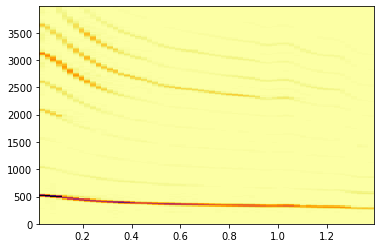
\includegraphics[scale=1]{fig/lab05/lab05_3.png}
		\caption{Спектрограмма звука}
	\end{center}
\end{figure}

Объеденим весь код из предыдущего пункта в одну функцию

\begin{lstlisting}[language=Python]
def estimate_fundamental(segment, low=50, high=200):
  lags, corrs = autocorr(segment)
  lag = np.array(corrs[low:high]).argmax() + low
  period = lag / segment.framerate
  frequency = 1 / period
  return frequency
\end{lstlisting}

\begin{lstlisting}[language=Python]
estimate_fundamental(segment1)
\end{lstlisting}
\begin{lstlisting}
364.4628099173554
\end{lstlisting}

Сделаем оценку высоты тона, применяя разделение на сегменты

\begin{lstlisting}[language=Python]
duration = wave.duration
step = 0.02
start = 0
time = []
frequencys = []
while start + step < duration:
  time.append(start + step/2)
  frequencys.append(estimate_fundamental(wave.segment(start=start,duration=step)))
  start += step
wave.make_spectrogram(2048).plot(high=900)
plt.plot(time, frequencys, color='black')
decorate(xlabel='Time (s)', ylabel='Frequency (Hz)')
\end{lstlisting}
\begin{figure}[H]
	\begin{center}
		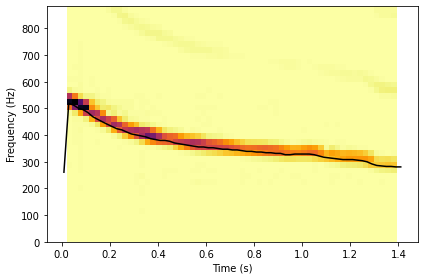
\includegraphics[scale=1]{fig/lab05/lab05_4.png}
		\caption{Результат оценки}
	\end{center}
\end{figure}

\subsection{Упражнение 3}

Вычислить автокорреляцию цен в платёжной системе Bitcoin. Оценить автокореляцию и проверить на признаки переодичности процесса.

\begin{lstlisting}[language=Python]
if not os.path.exists('market-pric.csv'):
    !wget https://github.com/Eugenepolyt/telecomunaction/raw/main/market-pric.csv

import pandas as pd
from thinkdsp import Wave

df = pd.read_csv('market-pric.csv', parse_dates=[0])
ys = df['market-price']
ts = df.index

w = Wave(ys, framerate=1)
w.plot()

\end{lstlisting}
\begin{figure}[H]
	\begin{center}
		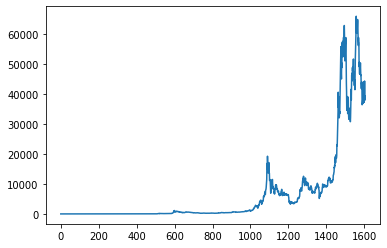
\includegraphics[scale=1]{fig/lab05/lab05_5.png}
		\caption{График цены на BitCoin}
	\end{center}
\end{figure}

Вычислим автокорреляцию:

\begin{lstlisting}[language=Python]
lags, corrs = autocorr(w)
plt.plot(lags, corrs)
decorate(xlabel='Lag',
        ylabel='Correlation')
\end{lstlisting}
\begin{figure}[H]
	\begin{center}
		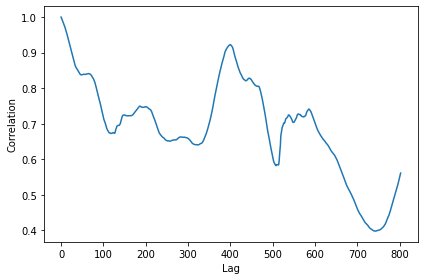
\includegraphics[scale=1]{fig/lab05/lab05_6.png}
		\caption{Автокорреляция функции цены на BitCoin}
	\end{center}
\end{figure}

По графику видно, что есть резкие спады и повышения. Процесс может напоминать переодичность.

\subsection{Упражнение 4}

В репозитории этой книги есть блокнот Jupyter под названием saxophone.ipynb, в котором исследуются автокорреляция, восприятие высоты тона и явление, называемое подавленная основная. Прочтите этот блокнот и «погоняйте» примеры. Выберите другой сегмент записи и вновь поработайте с примерами.

\begin{lstlisting}[language=Python]
if not os.path.exists('100475__iluppai__saxophone-weep.wav'):
    !wget https://github.com/AllenDowney/ThinkDSP/raw/master/code/100475__iluppai__saxophone-weep.wav
wave = read_wave('100475__iluppai__saxophone-weep.wav')
wave.normalize()
wave.make_audio()
spectrogram = wave.make_spectrogram(seg_length=1024)
spectrogram.plot(high=3000)
decorate(xlabel='Time (s)', ylabel='Frequency (Hz)')
\end{lstlisting}
\begin{figure}[H]
	\begin{center}
		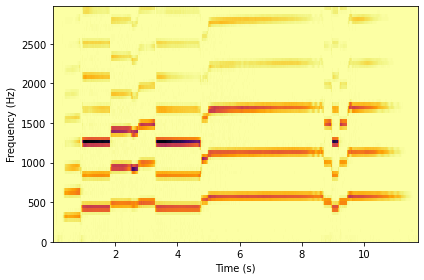
\includegraphics[scale=1]{fig/lab05/lab05_7.png}
		\caption{Спектрограмма сегмента}
	\end{center}
\end{figure}

Используем функции из блокнтота из репозитория и используем их для другого сегмента

\begin{lstlisting}[language=Python]
segment = wave.segment(start=4.0, duration=0.2)
segment.make_audio()
spectrum = segment.make_spectrum()
spectrum.plot(high=5000)
decorate(xlabel='Frequency', ylabel='Amplitude')
\end{lstlisting}

\begin{figure}[H]
	\begin{center}
		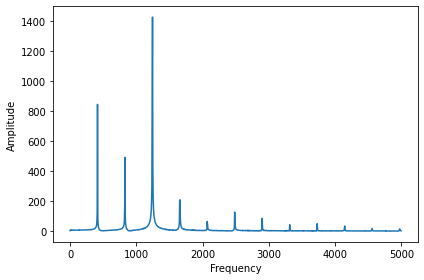
\includegraphics[scale=1]{fig/lab05/lab05_8.png}
		\caption{Спектр другого сегмента}
	\end{center}
\end{figure}

Пики в спектре находятся на 1245, 415 и 830 Гц

\begin{lstlisting}[language=Python]
spectrum.peaks()[:10]
\end{lstlisting}

\begin{lstlisting}
[(1425.371205417228, 1245.0),
 (844.1565084866448, 415.0),
 (810.3146734198679, 1240.0),
 (491.1468807713408, 830.0),
 (395.0157320768441, 1250.0),
 (285.5428668623747, 1235.0),
 (220.80813321938248, 1255.0),
 (208.75420107735613, 1660.0),
 (205.643155157793, 1655.0),
 (180.59606616391875, 1230.0)]
\end{lstlisting}

Сравним наш сегмент с треугольным сигналом

\begin{lstlisting}[language=Python]
from thinkdsp import TriangleSignal
TriangleSignal(freq=415).make_wave(duration=0.2).make_audio()
segment.make_audio()
\end{lstlisting}

У сигналов одинаковая воспринимаемая частота звука. Для понимания процесса восприятия основной частоты испольщуем АКФ.

\begin{lstlisting}[language=Python]
def autocorr2(segment):
    corrs = np.correlate(segment.ys, segment.ys, mode='same')
    N = len(corrs)
    lengths = range(N, N//2, -1)

    half = corrs[N//2:].copy()
    half /= lengths
    half /= half[0]
    return half

corrs = autocorr2(segment)
plt.plot(corrs[:500])
\end{lstlisting}

\begin{figure}[H]
	\begin{center}
		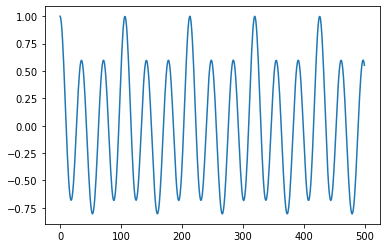
\includegraphics[scale=1]{fig/lab05/lab05_9.png}
		\caption{График после АКФ}
	\end{center}
\end{figure}

Первый пик находился возле lag 100

Найдём основную частоту при помощи написанной ранее функции.

\begin{lstlisting}[language=Python]
estimate_fundamental(segment)
\end{lstlisting}

\begin{lstlisting}
416.0377358490566
\end{lstlisting}

Воспринимаемая высота тона не изменится, если мы полностью удалим основной тон. Вот как выглядит спектр, если мы используем фильтр верхних частот, чтобы стереть основные частоты

\begin{lstlisting}[language=Python]
spectrum2 = segment.make_spectrum()
spectrum2.high_pass(600)
spectrum2.plot(high=3000)
decorate(xlabel='Frequency (Hz)', ylabel='Amplitude')
\end{lstlisting}

\begin{figure}[H]
	\begin{center}
		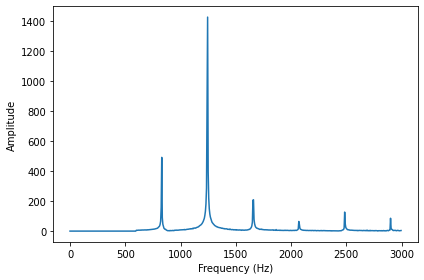
\includegraphics[scale=1]{fig/lab05/lab05_10.png}
		\caption{Спектр после ФНЧ}
	\end{center}
\end{figure}

Это явление называется "отсутствующим фундаментом"
Чтобы понять, почему мы слышим частоту, которой нет в сигнале, полезно взглянуть на функцию автокорреляции (ACF).

\begin{lstlisting}[language=Python]
corrs = autocorr2(segment2)
plt.plot(corrs[:500])
\end{lstlisting}

\begin{figure}[H]
	\begin{center}
		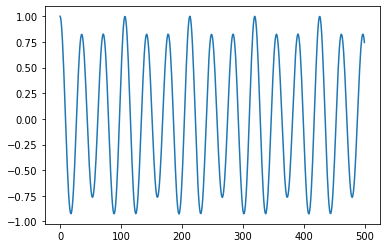
\includegraphics[scale=1]{fig/lab05/lab05_11.png}
		\caption{Полученный график}
	\end{center}
\end{figure}

\begin{lstlisting}[language=Python]
estimate_fundamental(segment)
\end{lstlisting}

\begin{lstlisting}
416.0377358490566
\end{lstlisting}

Таким образом, эти эксперименты показывают, что восприятие высоты тона основано не только на спектральном анализе, но и на чем-то вроде автокорреляции.

\subsection{Вывод}

В данной работе мы изучили корреляцию и как она влияет на сигналы, также был написан код для сигнала с "отсутствующим фунтаментом".


